\documentclass[11pt]{article} % use larger type; default would be 10pt

\usepackage[utf8]{inputenc} % set input encoding (not needed with XeLaTeX)
\usepackage{graphicx}
\usepackage{listings}
\usepackage{xcolor}

\usepackage{geometry} % to change the page dimensions
\geometry{a4paper} % or letterpaper (US) or a5paper or....

\usepackage{graphicx} % support the \includegraphics command and options

\usepackage{booktabs} % for much better looking tables
\usepackage{array} % for better arrays (eg matrices) in maths
\usepackage{paralist} % very flexible & customisable lists (eg. enumerate/itemize, etc.)
\usepackage{verbatim} % adds environment for commenting out blocks of text & for better verbatim
\usepackage{subfig} % make it possible to include more than one captioned figure/table in a single float

\usepackage{fancyhdr} % This should be set AFTER setting up the page geometry
\pagestyle{fancy} % options: empty , plain , fancy
\renewcommand{\headrulewidth}{0pt} % customise the layout...
\lhead{}\chead{}\rhead{}
\lfoot{}\cfoot{\thepage}\rfoot{}

\usepackage{sectsty}
\allsectionsfont{\sffamily\mdseries\upshape} % (See the fntguide.pdf for font help)
\usepackage[nottoc,notlof,notlot]{tocbibind} % Put the bibliography in the ToC
\usepackage[titles,subfigure]{tocloft} % Alter the style of the Table of Contents
\renewcommand{\cftsecfont}{\rmfamily\mdseries\upshape}
\renewcommand{\cftsecpagefont}{\rmfamily\mdseries\upshape} % No bold!


\title{Project Report}
\author{Group 18: Chengzhen Wu, Huiqi Mao, Ruofan Zhou}
%\date{} % Activate to display a given date or no date (if empty),
         % otherwise the current date is printed 

\begin{document}
\maketitle

\section{ER model}
After reading the feedback of diverable1, we modified our ER model as below:\\ \\
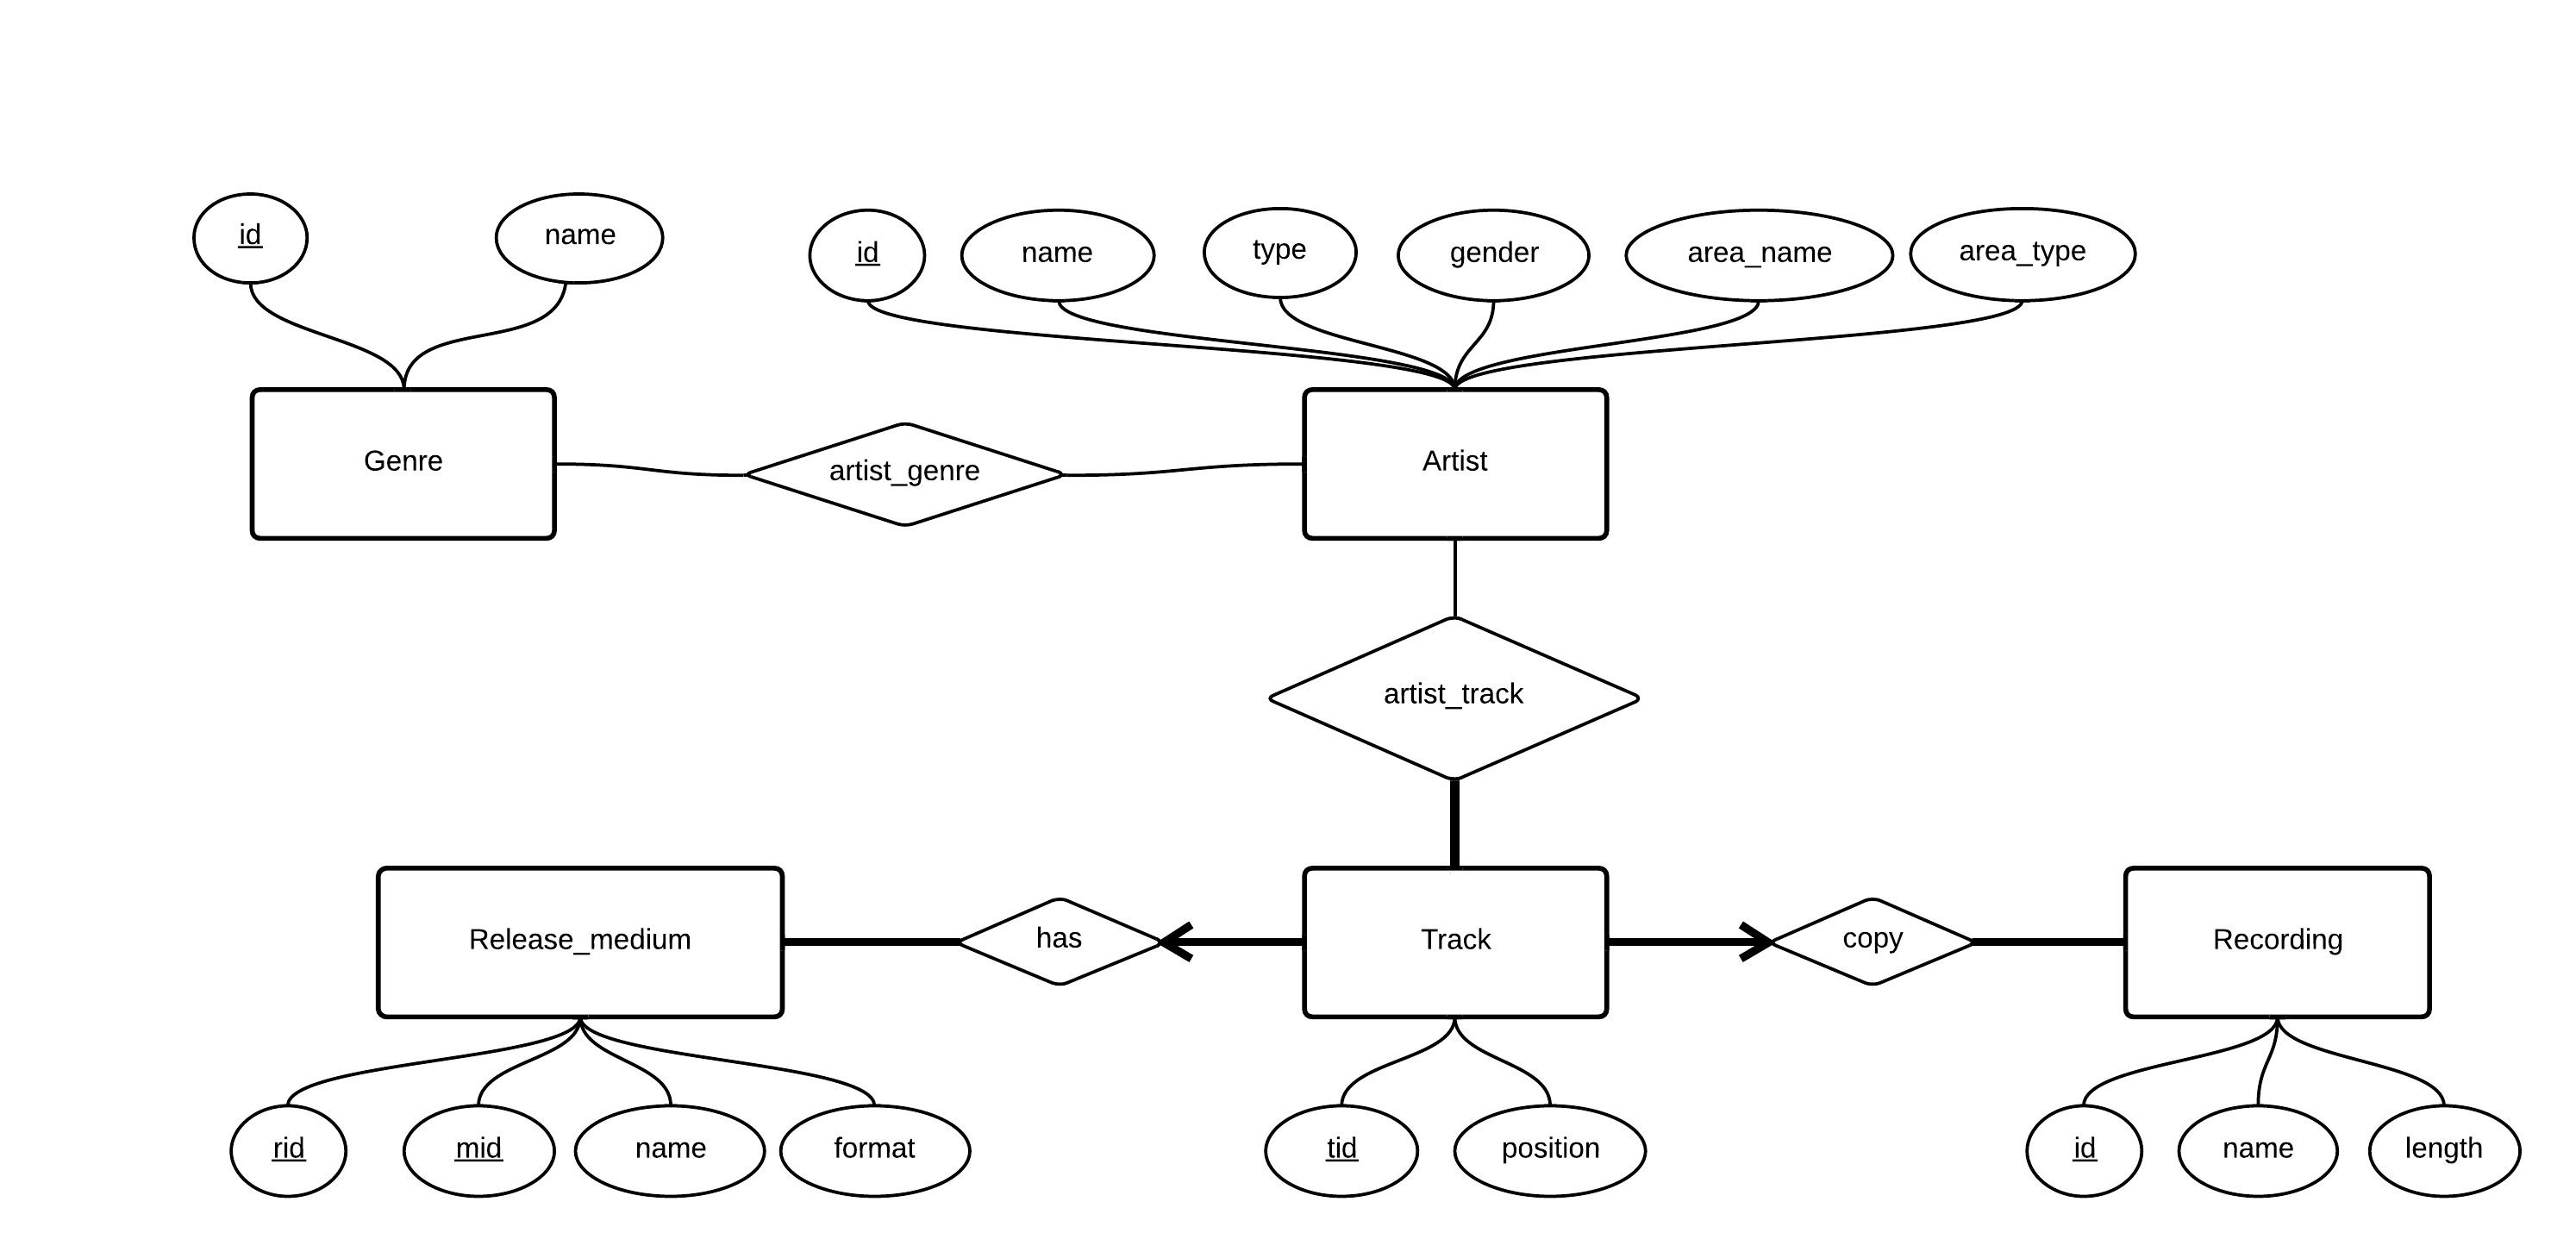
\includegraphics[width=14cm]{ERmodel}\\ \\
In the given project data, we firstly recognize 'area', 'artist' and 'genre' each as three individual entities. Each artist is from at most one area, so it's a many-to-one relation. Several artists can belong to different genres and one genre can contain several artists. So the relation between 'artist' and 'genre' is many-to-many.\\ \\
Secondly, we think about the relationship among 'release', 'recording', track' and 'medium'. We imagine a scene to describe these relations. The csv file of 'release' contains the names of releases. They could be stored in the mediums, such as CD, 12” Vinyl and so on. What's more, one release could have several CDs to contain many tracks, or in different medium (I'm not sure about this, but possible). So the relation between 'release' and 'medium' is one-to-many. Next, each track in different mediums must correspond to one recording. So the relation between 'track' and 'recording' is many-to-one. Each 'track' must be in one of 'medium's. So the relation is many-to-one.\\ \\
Finally, we merge one-to-may relations. 'release' and 'medium' are merged into 'Release\_medium'.  'area' can be merged into 'artist' as attributes. The 'has' relation between 'Release\_medium' and 'track' is merged into 'track' using 'mid' as foreign key. So is the 'copy' relation between 'recording' and 'track' using 'id' of recording as foreign key.\\ \\
Additionally, we ignore the 'count' in 'genre', which could be created as view in the database.\\ \\

\tiny{
\section{SQL based on ER model}
\begin{lstlisting}[language=SQL, keywordstyle=\color{blue!70},
commentstyle=\color{red!50!green!50!blue!50},
rulesepcolor=\color{red!20!green!20!blue!20},
frame=shadowbox]
--ENTITY Genre--
--we don't need gcount in genre
CREATE TABLE  Genre (
  ID Integer,
  name VARCHAR(300),
  PRIMARY KEY (ID)
  );

--ENTITY Artist--
CREATE TABLE  Artist (
  ID Integer,
  name VARCHAR(200),
  type CHAR(10),
  gender CHAR(6),
  area_name VARCHAR(150),
  area_type VARCHAR(15),
  PRIMARY KEY (ID)
  );
  
--ENTITY Recording--
CREATE TABLE  recording (
  ID Integer,
  name VARCHAR(2000),
  length VARCHAR(20),
  PRIMARY KEY (ID)
  );

--ENTITY RelaseMedium--
CREATE TABLE  ReleaseMedium (
  RID Integer NOT NULL,
  MID Integer,
  name VARCHAR(1000),
  format VARCHAR(45),
  PRIMARY KEY (MID)
  );

--ENTITY Track--
CREATE TABLE  Track (
  TID Integer,
  RCID Integer NOT NULL,
  MID Integer NOT NULL,
  position INTEGER,
  PRIMARY KEY (TID),
  FOREIGN KEY (MID) REFERENCES ReleaseMedium,
  FOREIGN KEY (RCID) REFERENCES Recording
  );
    
--RELATIONSHIP artist_genre
CREATE TABLE artist_genre (
  AID Integer NOT NULL,
  GID Integer NOT NULL,
  PRIMARY KEY (AID, GID),
  FOREIGN KEY (AID) REFERENCES Artist ON DELETE CASCADE,
  FOREIGN KEY (GID) REFERENCES Genre ON DELETE CASCADE
  );
    
--RELATIONSHIP artist_track
CREATE TABLE artist_track(
  AID Integer NOT NULL,
  TID Integer NOT NULL,
  PRIMARY KEY (AID, TID),
  FOREIGN KEY (AID) REFERENCES Artist,
  FOREIGN KEY (TID) REFERENCES Track
  );
\end{lstlisting}}

\normalsize{
\section{Queries}
We finished the queries based on our model: \\ \\
A
\begin{lstlisting}[language=SQL, keywordstyle=\color{blue!70},
commentstyle=\color{red!50!green!50!blue!50},
rulesepcolor=\color{red!20!green!20!blue!20},
frame=shadowbox]
select artist.NAME
  from ARTIST artist
  where artist.area_name='Switzerland';
\end{lstlisting}
B
\begin{lstlisting}[language=SQL, keywordstyle=\color{blue!70},
commentstyle=\color{red!50!green!50!blue!50},
rulesepcolor=\color{red!20!green!20!blue!20},
frame=shadowbox]
(select area_male.gender as type,
    area_male.area_name,area_male.sum as Number_of_Artist 
  from (
    select artist.gender,artist.AREA_NAME,count(*)as sum
      from ARTIST artist
      where artist.GENDER='Male' and artist.AREA_NAME <> 'null'
      GROUP BY artist.AREA_NAME, artist.gender
      order by count(*) desc) area_male
  where rownum = 1)
union
(select area_female.gender as type,
    area_female.area_name,area_female.sum as Number_of_Artist 
  from (
    select artist.gender,artist.AREA_NAME,count(*)as sum
      from ARTIST artist
      where artist.GENDER='Female' and artist.AREA_NAME <> 'null'
      GROUP BY artist.AREA_NAME, artist.gender
      order by count(*) desc)area_female
  where rownum = 1)
union
(select area_group.type as type,
    area_group.area_name,area_group.sum as Number_of_Artist 
  from (
    select artist.type,artist.AREA_NAME,count(*)as sum
      from ARTIST artist
      where artist.TYPE= 'Group' and artist.AREA_NAME <> 'null'
      GROUP BY artist.AREA_NAME, artist.gender, artist.type
      order by count(*) desc)area_group
  where rownum = 1);  
\end{lstlisting}
C
\begin{lstlisting}[language=SQL, keywordstyle=\color{blue!70},
commentstyle=\color{red!50!green!50!blue!50},
rulesepcolor=\color{red!20!green!20!blue!20},
frame=shadowbox]
select artist.name
  from (select artist.NAME,count(*)
    from artist artist,artist_track A_T
    where artist.type='Group' and A_T.aid=artist.id
    group by artist.name order by count(*) desc) artist
  where Rownum <= 10;
\end{lstlisting}
D
\begin{lstlisting}[language=SQL, keywordstyle=\color{blue!70},
commentstyle=\color{red!50!green!50!blue!50},
rulesepcolor=\color{red!20!green!20!blue!20},
frame=shadowbox]
select artist2.name
  from (
    select artist.id,artist.name
    from ARTIST artist
      join ARTIST_TRACK art_track on artist.ID = art_track.AID
      join TRACK track on art_track.TID = track.TID
      join RELEASEMEDIUM release_medium
          on track.MID = release_medium.MID
      where artist.type = 'Group'
      group by artist.id, artist.name
      order by count(*) desc) info, artist artist2
  WHERE rownum <= 10 and artist2.id = info.id;
\end{lstlisting}
E
\begin{lstlisting}[language=SQL, keywordstyle=\color{blue!70},
commentstyle=\color{red!50!green!50!blue!50},
rulesepcolor=\color{red!20!green!20!blue!20},
frame=shadowbox]
select artist.name
--project the artist name according to artist id
  from (
    select artist.id
      from artist artist, artist_genre art_genre, genre genre
      where artist.id = art_genre.aid
          and art_genre.GID = genre.ID
          and artist.gender = 'Female' 
      group by artist.id
      having count(*) = (
        select max(genre_count.count)
--find the maximum number of genre of a female artist
          from (
          select count(*)as count
            from artist artist2, artist_genre art_genre2,
                genre genre2
            where artist2.id = art_genre2.aid
                and art_genre2.GID = genre2.ID
                and artist2.gender = 'Female' 
            group by artist2.id) genre_count))max_count,
                artist artist
  where artist.id = max_count.ID;
\end{lstlisting}
F
\begin{lstlisting}[language=SQL, keywordstyle=\color{blue!70},
commentstyle=\color{red!50!green!50!blue!50},
rulesepcolor=\color{red!20!green!20!blue!20},
frame=shadowbox]
select female_count.area_name
  from (
    select artist.area_name, count(*)as count
      from artist artist
      where artist.AREA_TYPE='City' and gender ='Male'
      group by artist.area_name, artist.gender) male_count,
      (select artist.area_name, count(*)as count
        from artist artist
        where artist.AREA_TYPE='City' and gender ='Female'
        group by artist.area_name, artist.gender) female_count
  where male_count.area_name = female_count.area_name and 
      female_count.count > male_count.count;
\end{lstlisting}
G
\begin{lstlisting}[language=SQL, keywordstyle=\color{blue!70},
commentstyle=\color{red!50!green!50!blue!50},
rulesepcolor=\color{red!20!green!20!blue!20},
frame=shadowbox]
create view med_track as
  select release_medium.MID,count(*) as tracks
    from ReleaseMedium release_medium,TRACK track
    where track.MID = release_medium.MID
    group by release_medium.MID order by count(*) desc;

select med_track.mid
  from  med_track 
  where med_track.tracks =
      (select MAX(med_track.tracks)
                         from  med_track);
\end{lstlisting}
H
\begin{lstlisting}[language=SQL, keywordstyle=\color{blue!70},
commentstyle=\color{red!50!green!50!blue!50},
rulesepcolor=\color{red!20!green!20!blue!20},
frame=shadowbox]
select lst.area_name, lst.name
  from (
  select artist.area_name,artist.name, rank() over
      (partition by artist.area_name
      order by count(*) desc) as rank
    from artist_track at1, (
      select artist.area_name,artist.id ,artist.name
        from ARTIST artist where artist.gender = 'Male') artist
        where artist.id =at1.AID and artist.area_name in (
          select a1.area_name
            from artist a1 
            where a1.area_name is not null
            group by a1.area_name
            having count(*)>30)
       group by artist.area_name, artist.id,artist.name) lst
    where lst.rank = 1
union
select lst.area_name, lst.name
  from (
    select artist.area_name,artist.name, rank() over
        (partition by artist.area_name
        order by count(*) desc) as rank
    from artist_track at1, (
    select artist.area_name,artist.id ,artist.name
      from ARTIST artist where artist.gender = 'Female') artist
      where artist.id =at1.AID and artist.area_name in (
        select a1.area_name
          from artist a1 
          where a1.area_name is not null
          group by a1.area_name
          having count(*)>30)
     group by artist.area_name, artist.id,artist.name) lst
  where lst.rank = 1
union
select lst.area_name, lst.name
  from (
    select artist.area_name,artist.name, rank() over
        (partition by artist.area_name
        order by count(*) desc) as rank
      from artist_track at1, (
      select artist.area_name,artist.id ,artist.name
        from ARTIST artist where artist.type = 'Group') artist
        where artist.id =at1.AID and artist.area_name in (
        select a1.area_name
          from artist a1 
          where a1.area_name is not null
          group by a1.area_name
          having count(*)>30)
      group by artist.area_name, artist.id,artist.name) lst
  where lst.rank = 1;
\end{lstlisting}
I
\begin{lstlisting}[language=SQL, keywordstyle=\color{blue!70},
commentstyle=\color{red!50!green!50!blue!50},
rulesepcolor=\color{red!20!green!20!blue!20},
frame=shadowbox]
select recording.name
  from RECORDING ,(
  select track.rcid, rank()
      over (order by count(distinct track.mid) desc) as rank
    from TRACK track
    where exists (
      select artrack.TID
        from ARTIST artist, ARTIST_TRACK artrack
        where artist.name = 'Metallica'
            and  artrack.aid=artist.id
            and track.tid = artrack.tid)
    group by track.rcid) toptrak 
  where toptrak.rank<=25 and recording.id = toptrak.rcid;
\end{lstlisting}
J
\begin{lstlisting}[language=SQL, keywordstyle=\color{blue!70},
commentstyle=\color{red!50!green!50!blue!50},
rulesepcolor=\color{red!20!green!20!blue!20},
frame=shadowbox]
select genre.NAME, artistrank.NAME
  from genre ,(
  select artistfilter.GID,artistfilter.NAME, rank()
    over (PARTITION BY artistfilter.GID ORDER by count(*) desc)
        as rank
    from artist_track at1, (
    select artist.ID, topgenreartist.GID, artist.NAME
      from artist , (
      select ag2.AID, ag2.GID
       from artist_genre ag2 ,(
       select ag1.gid as gid, rank() over (order by count(*) desc)
           as rank
         from Artist_GENRE ag1
         group by ag1.gid) genrelst
       where ag2.gid = genrelst.gid
           and genrelst.rank<=10) topgenreartist
      where artist.gender = 'Female'
          and artist.id = topgenreartist.aid)artistfilter
    where artistfilter.id = at1.aid
    group by artistfilter.gid,
        at1.aid,artistfilter.NAME)artistrank
  where artistrank.rank = 1 and genre.ID=artistrank.GID;
\end{lstlisting}
K
\begin{lstlisting}[language=SQL, keywordstyle=\color{blue!70},
commentstyle=\color{red!50!green!50!blue!50},
rulesepcolor=\color{red!20!green!20!blue!20},
frame=shadowbox]
(select distinct genre1.name
  from genre genre1)
--get the list of all genres
minus
(select distinct genre.NAME
  from genre genre, artist_genre artist_genre, artist artist
  where genre.ID = artist_genre.GID
       and artist.ID = artist_genre.AID
       and artist.gender = 'Female');
--change 'Female' to 'Male'\artist.type='Group'
\end{lstlisting}
L
\begin{lstlisting}[language=SQL, keywordstyle=\color{blue!70},
commentstyle=\color{red!50!green!50!blue!50},
rulesepcolor=\color{red!20!green!20!blue!20},
frame=shadowbox]
select *
  from (
  select MaleArtist.area_name ,
      MaleArtist.id, count(*), rank()
      over (Partition by MaleArtist.area_name
      order by count(artist_track.tid))as rank
    from artist_track artist_track,(
      select artist.id, artist.name, artist.area_name
        from artist, (
        select artist.area_name
          from artist
          where artist.type = 'Group'
              and artist.area_name is not null
          group by artist.area_name
          having count(*)>10) arealist
        where artist.area_name  = arealist.area_name
            and artist.gender = 'Male') MaleArtist
      where artist_track.aid = MaleArtist.id 
      group by MaleArtist.area_name,MaleArtist.id)
  where rank<=5;
\end{lstlisting}
M
\begin{lstlisting}[language=SQL, keywordstyle=\color{blue!70},
commentstyle=\color{red!50!green!50!blue!50},
rulesepcolor=\color{red!20!green!20!blue!20},
frame=shadowbox]
create view compilation as
  select track.mid
    from track ,artist_track at1
    where track.tid = at1.tid
    group by track.mid
    having count(distinct at1.aid)>1;

select *
  from (
  select  artist.name
    from artist  join (
    select ct.tid, artist_track.aid
      from (
      select t.tid
        from track t join compilation c on t.mid = c.mid) ct
        join artist_track on ct.tid = artist_track.tid) cta
      on artist.id = cta.aid 
      where artist.type = 'Group'
      group by artist.id, artist.name
    order by count(*) desc)
  where ROWNUM<=10;
\end{lstlisting}
N
\begin{lstlisting}[language=SQL, keywordstyle=\color{blue!70},
commentstyle=\color{red!50!green!50!blue!50},
rulesepcolor=\color{red!20!green!20!blue!20},
frame=shadowbox]
create view ReleaseTrack as
  select ReleaseMedium.rid,track.tid
    from ReleaseMedium join track on
        track.mid = releasemedium.mid;

create view album as
  select R.rid, R.tid
    from ReleaseTrack R
    where exists (
    select artist.id
      from artist
        where not exists (
        select A_T.aid
          from Artist_Track A_T
          where A_T.aid <> Artist.id and A_T.tid = R.tid));
              
select colla.rid
  from (
  select album.rid
    from album, artist_track at1
    where album.tid = at1.tid
    group by album.rid
    order by count(distinct at1.aid) desc) colla
  where rownum<=10;
\end{lstlisting}
O
\begin{lstlisting}[language=SQL, keywordstyle=\color{blue!70},
commentstyle=\color{red!50!green!50!blue!50},
rulesepcolor=\color{red!20!green!20!blue!20},
frame=shadowbox]
select R.name
  from ReleaseMedium R
  group by R.rid , R.name
  having count(*) = (
    select max(RM.count)
      from(
      select ReleaseMedium.rid, count(*) as count
        from ReleaseMedium
        group by ReleaseMedium.rid
    ) RM
  );
\end{lstlisting}
P
\begin{lstlisting}[language=SQL, keywordstyle=\color{blue!70},
commentstyle=\color{red!50!green!50!blue!50},
rulesepcolor=\color{red!20!green!20!blue!20},
frame=shadowbox]
select genre_name.name
  from (
  select artist_genre2.gid, count(*)as count
    from (
    select artist.id
      from genre genre, artist artist, artist_genre artist_genre
      where artist.type ='Group' and genre.id = artist_genre.gid
          and artist_genre.aid = artist.id
      group by artist.id
      having count(*)>=3)groupid, artist_genre artist_genre2
    where artist_genre2.aid = groupid.id
    group by artist_genre2.gid) lst,genre genre_name
  where genre_name.id = lst.gid
      and lst.count = (
    SELECT max(gid_count.count)
--find the count of the most popular genre first
      FROM (
      select artist_genre2.gid, count(*)as count
        from (
        select artist.id
          from genre genre, artist artist,
              artist_genre artist_genre
          where artist.type ='Group'
              and genre.id = artist_genre.gid
              and artist_genre.aid = artist.id
          group by artist.id
          having count(*)>=3)groupid, artist_genre artist_genre2
        where artist_genre2.aid = groupid.id
        group by artist_genre2.gid) gid_count
     );
\end{lstlisting}
Q
\begin{lstlisting}[language=SQL, keywordstyle=\color{blue!70},
commentstyle=\color{red!50!green!50!blue!50},
rulesepcolor=\color{red!20!green!20!blue!20},
frame=shadowbox]
select *
  from(
  select recording.name, count(*)
    from recording recording
    where recording.id<1000000
        and recording.name not like '[%]'
--get rid of [untitled] or[unknown] etc.
    group by recording.name
    order by count(*) desc)
  where rownum<=5;
\end{lstlisting}
R
\begin{lstlisting}[language=SQL, keywordstyle=\color{blue!70},
commentstyle=\color{red!50!green!50!blue!50},
rulesepcolor=\color{red!20!green!20!blue!20},
frame=shadowbox]
--artist_count_track is a table with artist id
--    and the number of tracks he has.
--artist_count_release is a table with artist id
--    and the number of releases his track has contributed to.
--join2 simply join the above two tables together
--    in order to caculate the ratio in the next step

create view artist_count_track as
  select artist_track.aid, count(*) as track_count
    from artist_track artist_track
    group by artist_track.aid;
            
create view artist_count_release as            
  select join1.aid, count(distinct releasemedium.rid)
      as release_count
    from (
    select artist_track.aid, track.mid
      from artist_track artist_track, track track
      where artist_track.tid = track.tid) join1,
          releasemedium releasemedium
    where join1.mid = releasemedium.mid
    group by join1.aid;
             
select artist.name
  from (
  select count_t.aid
    from artist_count_track count_t,
        artist_count_release count_r
    where count_t.aid = count_r.aid
    order by (count_t.track_count/count_r.release_count)
        desc)join2, artist artist
  where rownum <=10 and artist.id = join2.aid;
--select the top 10 and get the artist name from artist id
\end{lstlisting}
S
\begin{lstlisting}[language=SQL, keywordstyle=\color{blue!70},
commentstyle=\color{red!50!green!50!blue!50},
rulesepcolor=\color{red!20!green!20!blue!20},
frame=shadowbox]
create view hittrack as
  select t.rcid
  from track t
  group by t.rcid
  having count(distinct t.mid)>100;

create view htid as
  select t.tid, t.rcid
  from track t, hittrack ht
  where t.rcid = ht.rcid;

create view hitartist as
  select at1.aid
  from artist_track at1,htid t
  where t.tid = at1.tid
  group by at1.aid
  having count(distinct t.rcid)>10;

create view hitability as
  select lst.aid , sum(lst.count) as score
  from (
  select hiat.aid, t.rcid ,count(distinct t.mid)
      as count, rank() over (partition by hiat.aid
      order by count(distinct t.mid) desc) as rank
    from track t,(
    select hta.aid,at1.tid
      from hitartist hta, artist_track at1
      where hta.aid = at1.aid) hiat
      where t.tid = hiat.tid
      group by hiat.aid,t.rcid 
      having count(distinct t.mid)>100) lst
    where lst.rank<=10 
    group by lst.aid;

select artist.name, ab.score
  from hitartist art , hitability ab,artist
  where art.aid = ab.aid and artist.id = art.aid;

\end{lstlisting}

\section{Analyze the Queries}

We've already created 8 indexes:\\
\begin{lstlisting}[language=SQL, keywordstyle=\color{blue!70},
commentstyle=\color{red!50!green!50!blue!50},
rulesepcolor=\color{red!20!green!20!blue!20},
frame=shadowbox]
create bitmap index genderindex
on  artist(gender); 

create bitmap index typeindex
on artist(type);

create bitmap index areaindex
on artist(area_name);

create index nameindex
on artist(name);

create index artrack
on  artist_track(aid);

create index artracktid
on  artist_track(tid);

create index genreindex
on artist_genre(gid);

create index tracktid
on track(mid);
\end{lstlisting}

We choosed Query H, Query I and Query J.

\subsection{Query H}

An AID-index is built on TABLE artist\_track because it can speed up the range scan(In the SQL, we used only AID for this TABLE, so it's obvious that we should use this index).\\
There is a bitmap index built on area\_name for TABLE artist to quickly group the artists by attribute "area\_name". It will take much more time to grasp the number of artists in every area if we don't have this index (there are 264690 areas and 815387 artists, thus may cost about O($10^{10}$) for grouping without area-indexing). \\
The system also used the bitmap index on gender for TABLE artist, since bitmap indexes are compact and they work best for columns with a small set of values(the attribute "gender" contains only 3 kinds of value: "Male", "Female" and "Other"). Then we can quickly partition artists from areas by gender. \\
Finally, we succeeded in running the query in \textbf{about 30s}. The join(artist and artist\_track) takes most of time(60\%+ of IO cost) since both contain a large amount of data, and relatively little time with group(by gender and area\_name, about 20\% IO cost) when we use the indexes.\\
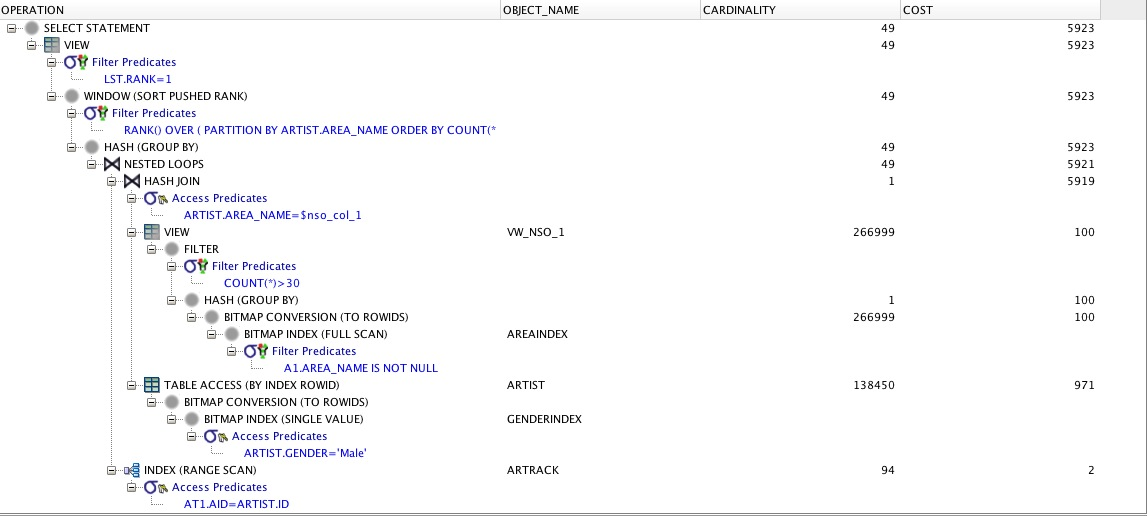
\includegraphics[width=14cm]{costh}

\subsection{Query I}
The indexes are built on attribute name on for TABLE artist, and indexes of tables of their own. In the plan explaition, we can see that all IO cost by table access is very little thanks to the indexes.\\
We ran the query in \textbf{539 ms}. The "exists" cost most of the IO cost.\\
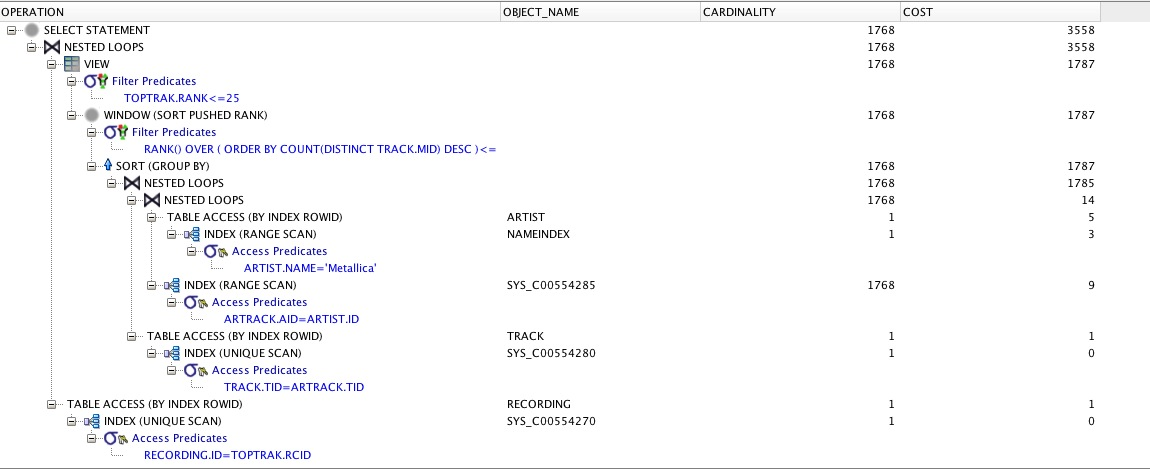
\includegraphics[width=14cm]{costi}

\subsection{Query J}
The indexes used are gender-index on TABLE artist and gid-index on TABLE genre. For gender-index, we've already discuessed in anlysis for Query H. And for gid-index, it managed to fast-full scan for the "group by gid". Thus, the indexes are important when we do such kind of queries(especially for "GROUP BY").\\
The query cost \textbf{7270 ms}. 50% of the IO cost is on the "join"(it's foreseeable since it really cost when we need to join the 2 large tables), and another 50% of the IO cost is on the outer "GROUP BY" (since the cardinality is very large). Other part of the query(table access, inner group by and select) cost very little.
\\
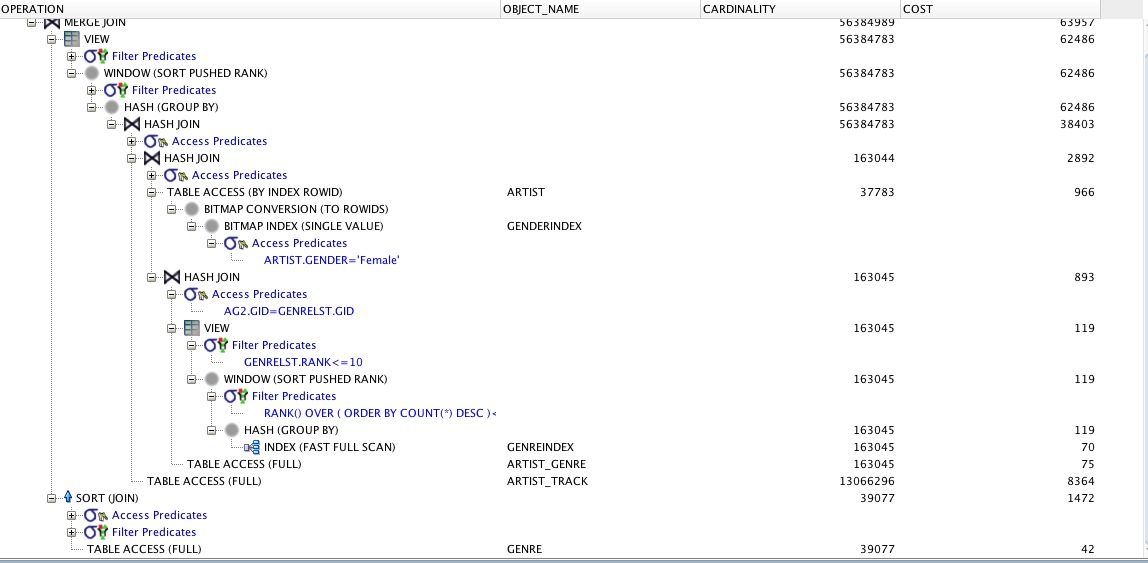
\includegraphics[width=14cm]{costj}


\section{Interface}
Since we've already upload the data to the server, it's convient for us to use PHP + Apache + Oracle to build the website as interface, like below:\\ \\
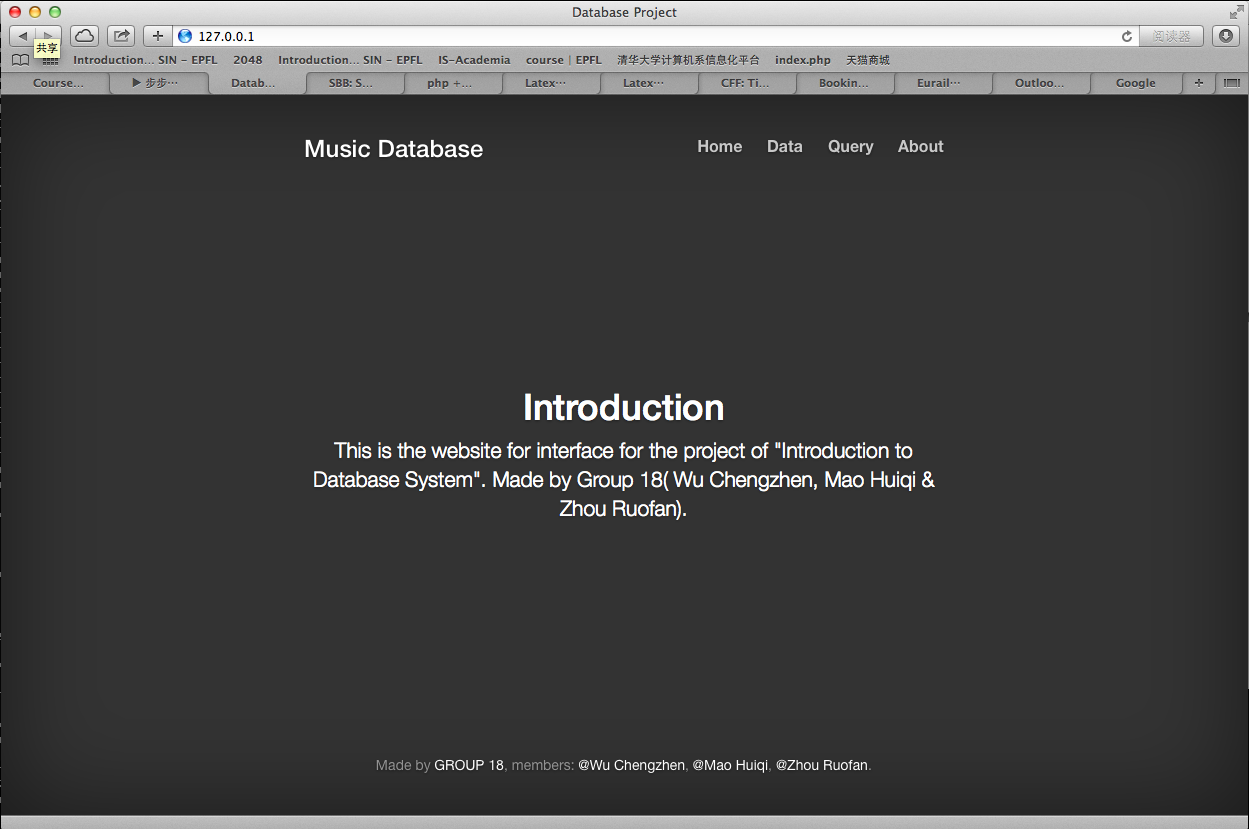
\includegraphics[width=14cm]{interface1}\\ \\
It's the index of our website. The website contains 4 parts: Home, Data, Query and About, and the functionally page is Data and Query.\\ \\
The screen shot of Data page is as below, the page shows the data of tables(you can select the table you want to see by clicking the link of table names, which are the yellow words on the uper part of the page). Each page would show 20 data and you can blowse more data by click the link of pages on the bottom part of the page. As the screen shot, it shows the 'artist' table. By moving your mouse onto those foreign keys, a prompt box showing the message of the table linked by the foreign key or relationship(as the screen shot, we move the mouse onto the 'genre' and a box showing message of the genre name and genre id of the artist).\\ \\
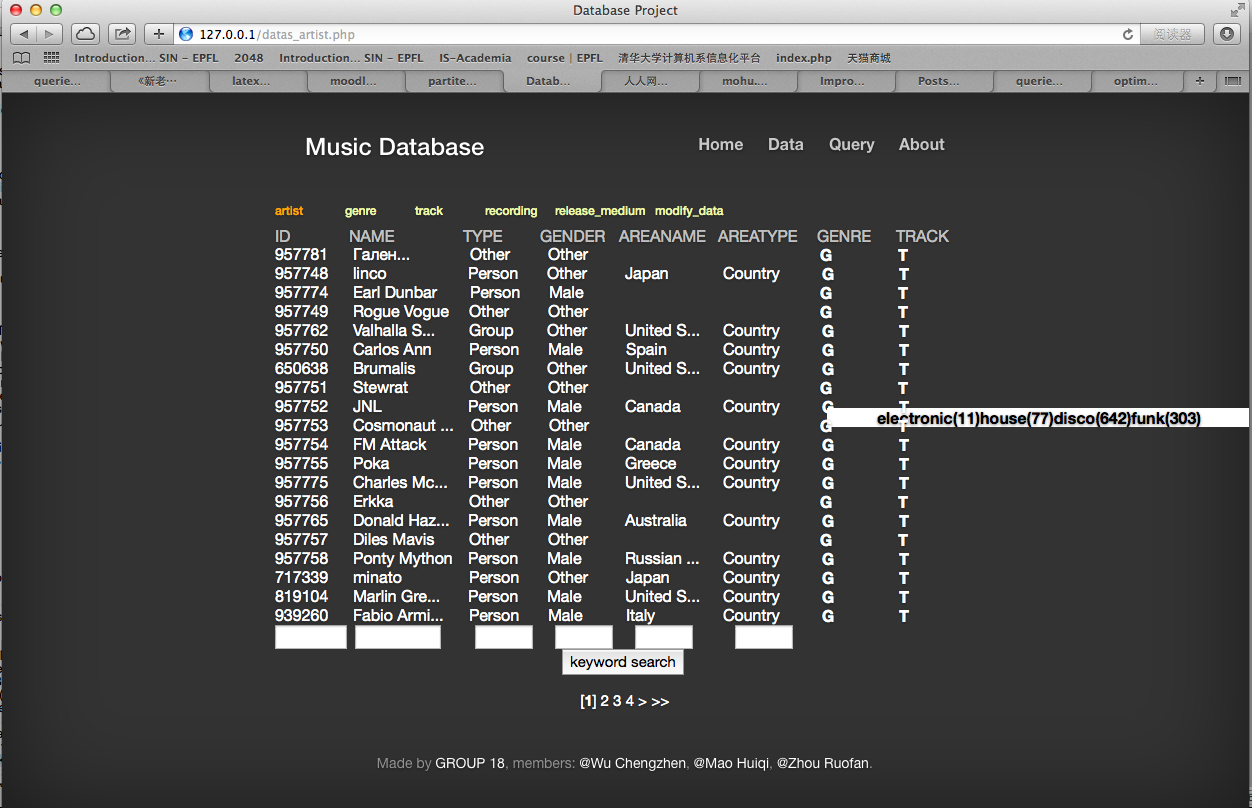
\includegraphics[width=13cm]{interface2}\\ \\
Under each row there's a input box, and you can use it to search for keyword. Just by clicking the "Keyword Search" you can filter the data of the table. For example, next screen shot shows the result as we input 'China' and 'Female' under keyword 'AREA\_NAME' and 'GENDER'. \\ \\
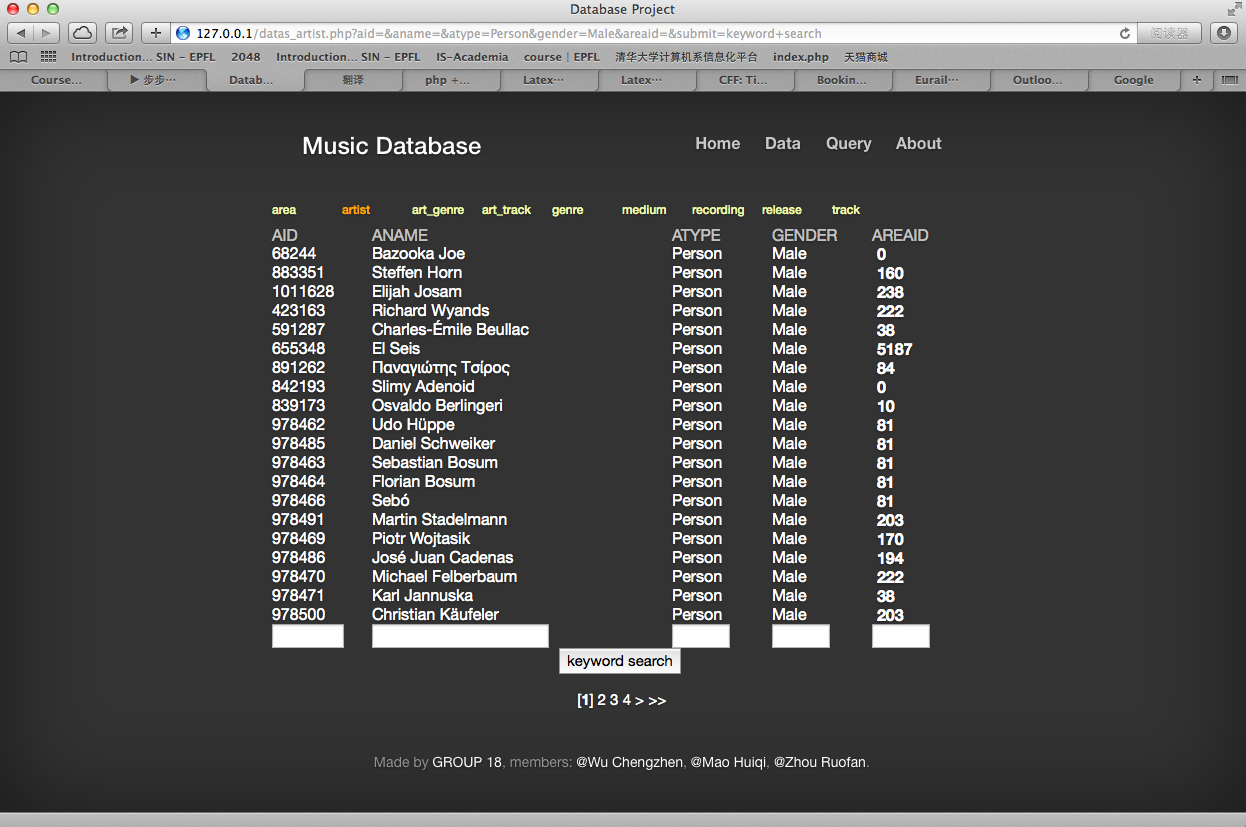
\includegraphics[width=13cm]{interface3}\\ \\
And in the data\_modify page, we implement the insert and delete of data. Once given paremeters and clicked "run", the SQL ran will be printed and the SQL will be executed. The result is as below. We've already tested and this function is available.\\ \\
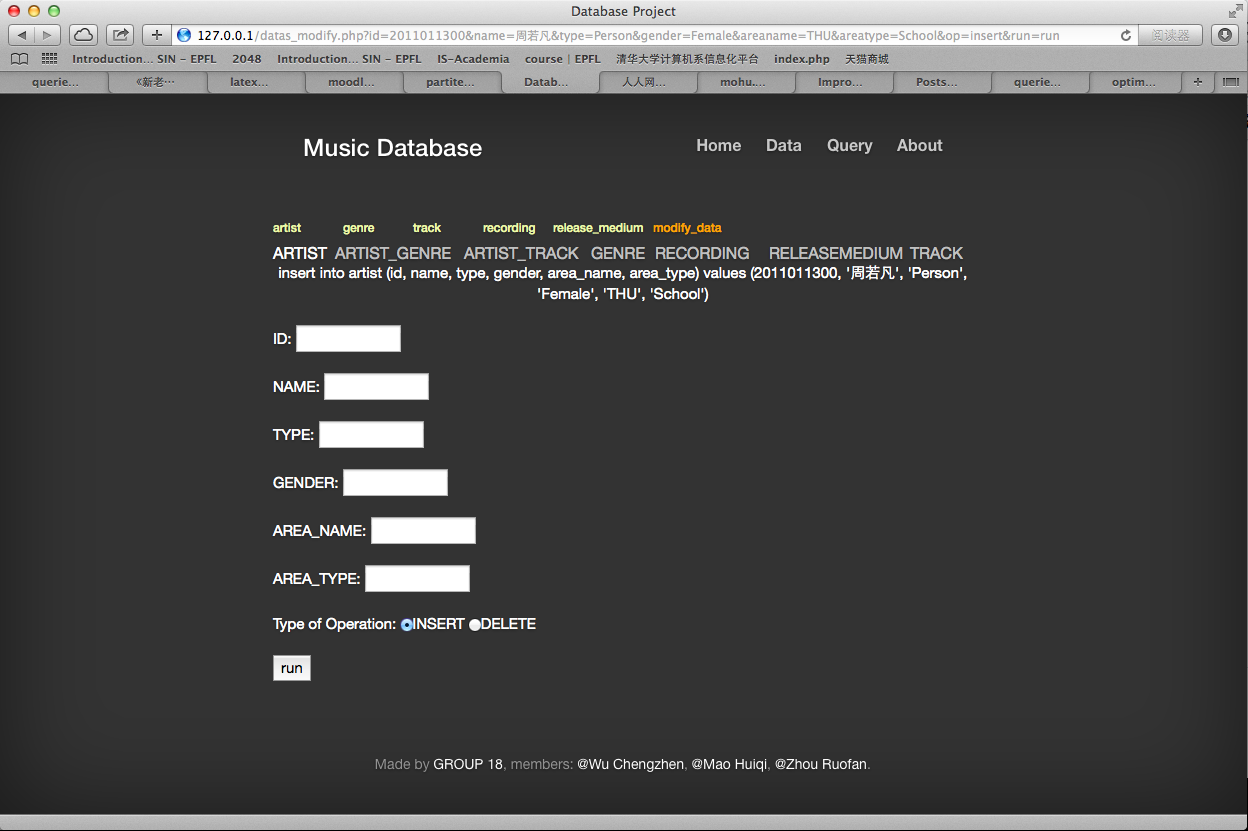
\includegraphics[width=13cm]{interface5}\\ \\
And we satisfied all the queries(A-S) in the Query page, and you can see the results by clicking the query number.\\ \\
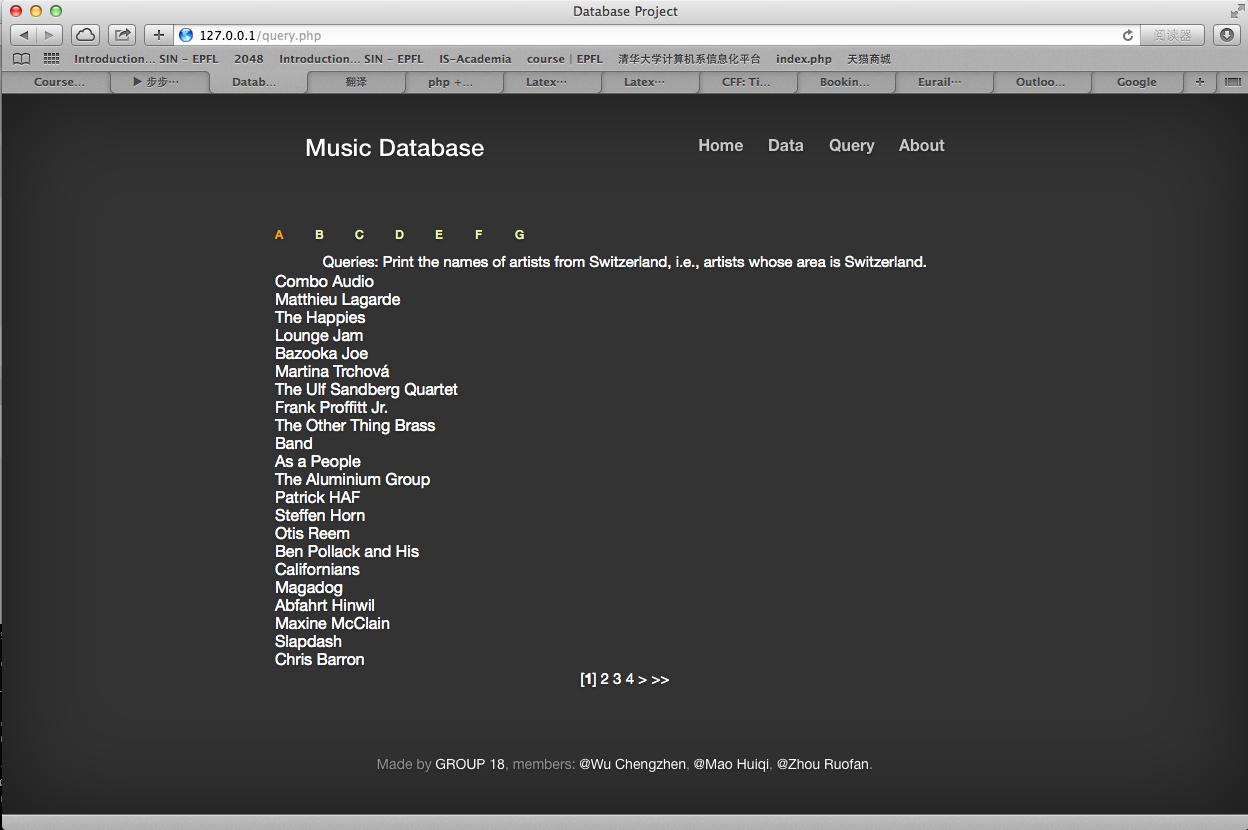
\includegraphics[width=10cm]{interface4}\\ \\
}

\end{document}
